\documentclass[ignorenonframetext,]{beamer}
\setbeamertemplate{caption}[numbered]
\setbeamertemplate{caption label separator}{: }
\setbeamercolor{caption name}{fg=normal text.fg}
\beamertemplatenavigationsymbolsempty
\usepackage{lmodern}
\usepackage{amssymb,amsmath}
\usepackage{ifxetex,ifluatex}
\usepackage{fixltx2e} % provides \textsubscript
\ifnum 0\ifxetex 1\fi\ifluatex 1\fi=0 % if pdftex
  \usepackage[T1]{fontenc}
  \usepackage[utf8]{inputenc}
\else % if luatex or xelatex
  \ifxetex
    \usepackage{mathspec}
  \else
    \usepackage{fontspec}
  \fi
  \defaultfontfeatures{Ligatures=TeX,Scale=MatchLowercase}
\fi
% use upquote if available, for straight quotes in verbatim environments
\IfFileExists{upquote.sty}{\usepackage{upquote}}{}
% use microtype if available
\IfFileExists{microtype.sty}{%
\usepackage{microtype}
\UseMicrotypeSet[protrusion]{basicmath} % disable protrusion for tt fonts
}{}
\newif\ifbibliography
\hypersetup{
            pdftitle={Introduction to R},
            pdfborder={0 0 0},
            breaklinks=true}
\urlstyle{same}  % don't use monospace font for urls
\usepackage{graphicx,grffile}
\makeatletter
\def\maxwidth{\ifdim\Gin@nat@width>\linewidth\linewidth\else\Gin@nat@width\fi}
\def\maxheight{\ifdim\Gin@nat@height>\textheight0.8\textheight\else\Gin@nat@height\fi}
\makeatother
% Scale images if necessary, so that they will not overflow the page
% margins by default, and it is still possible to overwrite the defaults
% using explicit options in \includegraphics[width, height, ...]{}
\setkeys{Gin}{width=\maxwidth,height=\maxheight,keepaspectratio}

% Prevent slide breaks in the middle of a paragraph:
\widowpenalties 1 10000
\raggedbottom

\AtBeginPart{
  \let\insertpartnumber\relax
  \let\partname\relax
  \frame{\partpage}
}
\AtBeginSection{
  \ifbibliography
  \else
    \let\insertsectionnumber\relax
    \let\sectionname\relax
    \frame{\sectionpage}
  \fi
}
\AtBeginSubsection{
  \let\insertsubsectionnumber\relax
  \let\subsectionname\relax
  \frame{\subsectionpage}
}

\setlength{\parindent}{0pt}
\setlength{\parskip}{6pt plus 2pt minus 1pt}
\setlength{\emergencystretch}{3em}  % prevent overfull lines
\providecommand{\tightlist}{%
  \setlength{\itemsep}{0pt}\setlength{\parskip}{0pt}}
\setcounter{secnumdepth}{0}

\title{Introduction to R}
\date{}

\begin{document}
\frame{\titlepage}

\begin{frame}{Background (Wikipedia)}

``R is an open source programming language and software environment for
statistical computing and graphics that is supported by the R Foundation
for Statistical Computing.

The R language is widely used among statisticians and data miners for
developing statistical software and data analysis.``''

\end{frame}

\begin{frame}{R is}

\begin{itemize}[<+->]
\tightlist
\item
  a programming language
\item
  a statistical package
\item
  open source
\end{itemize}

\end{frame}

\begin{frame}{R is not}

\begin{itemize}[<+->]
\tightlist
\item
  a database
\item
  a spreadsheet
\item
  commercially supported
\end{itemize}

\end{frame}

\begin{frame}{Advantages of R}

\begin{itemize}[<+->]
\tightlist
\item
  It's free
\item
  It's powerful
\item
  It's popular
\end{itemize}

\end{frame}

\begin{frame}

\begin{block}{}

\begin{figure}
\centering
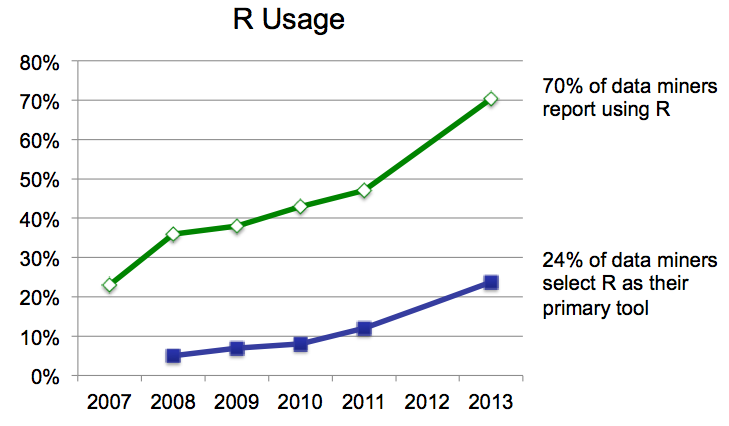
\includegraphics{C:/HillsdaleR/RUsage.png}
\caption{Source: Revolution Analytics}
\end{figure}

\end{block}

\end{frame}

\begin{frame}{Disadvantages of R}

It can be frustrating.

\begin{block}{}

\emph{}

\end{block}

\end{frame}

\section{Questions?}\label{questions}

\end{document}
